% Created by tikzDevice version 0.12 on 2018-09-28 04:17:32
% !TEX encoding = UTF-8 Unicode
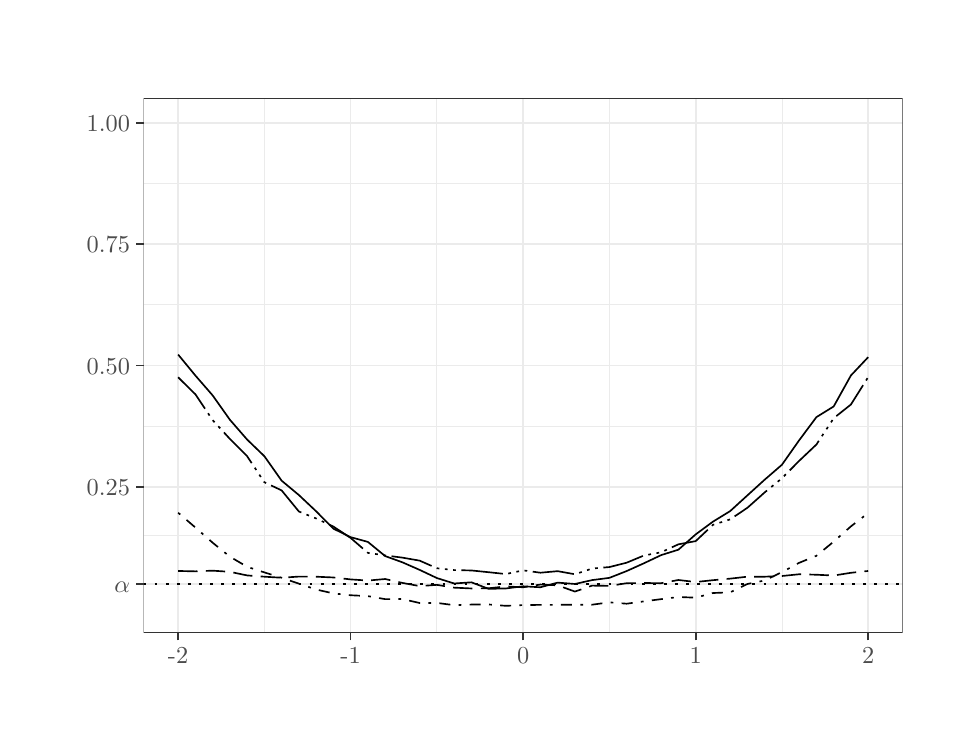
\begin{tikzpicture}[x=1pt,y=1pt]
\definecolor{fillColor}{RGB}{255,255,255}
\path[use as bounding box,fill=fillColor,fill opacity=0.00] (0,0) rectangle (325.21,252.94);
\begin{scope}
\path[clip] (  0.00,  0.00) rectangle (325.21,252.94);
\definecolor{drawColor}{RGB}{255,255,255}
\definecolor{fillColor}{RGB}{255,255,255}

\path[draw=drawColor,line width= 0.6pt,line join=round,line cap=round,fill=fillColor] (  0.00,  0.00) rectangle (325.21,252.94);
\end{scope}
\begin{scope}
\path[clip] ( 41.90, 34.26) rectangle (316.18,227.38);
\definecolor{fillColor}{RGB}{255,255,255}

\path[fill=fillColor] ( 41.90, 34.26) rectangle (316.18,227.38);
\definecolor{drawColor}{gray}{0.92}

\path[draw=drawColor,line width= 0.3pt,line join=round] ( 41.90, 69.37) --
	(316.18, 69.37);

\path[draw=drawColor,line width= 0.3pt,line join=round] ( 41.90,108.87) --
	(316.18,108.87);

\path[draw=drawColor,line width= 0.3pt,line join=round] ( 41.90,152.76) --
	(316.18,152.76);

\path[draw=drawColor,line width= 0.3pt,line join=round] ( 41.90,196.65) --
	(316.18,196.65);

\path[draw=drawColor,line width= 0.3pt,line join=round] ( 85.53, 34.26) --
	( 85.53,227.38);

\path[draw=drawColor,line width= 0.3pt,line join=round] (147.87, 34.26) --
	(147.87,227.38);

\path[draw=drawColor,line width= 0.3pt,line join=round] (210.21, 34.26) --
	(210.21,227.38);

\path[draw=drawColor,line width= 0.3pt,line join=round] (272.55, 34.26) --
	(272.55,227.38);

\path[draw=drawColor,line width= 0.6pt,line join=round] ( 41.90, 51.81) --
	(316.18, 51.81);

\path[draw=drawColor,line width= 0.6pt,line join=round] ( 41.90, 86.93) --
	(316.18, 86.93);

\path[draw=drawColor,line width= 0.6pt,line join=round] ( 41.90,130.82) --
	(316.18,130.82);

\path[draw=drawColor,line width= 0.6pt,line join=round] ( 41.90,174.71) --
	(316.18,174.71);

\path[draw=drawColor,line width= 0.6pt,line join=round] ( 41.90,218.60) --
	(316.18,218.60);

\path[draw=drawColor,line width= 0.6pt,line join=round] ( 54.37, 34.26) --
	( 54.37,227.38);

\path[draw=drawColor,line width= 0.6pt,line join=round] (116.70, 34.26) --
	(116.70,227.38);

\path[draw=drawColor,line width= 0.6pt,line join=round] (179.04, 34.26) --
	(179.04,227.38);

\path[draw=drawColor,line width= 0.6pt,line join=round] (241.38, 34.26) --
	(241.38,227.38);

\path[draw=drawColor,line width= 0.6pt,line join=round] (303.71, 34.26) --
	(303.71,227.38);
\definecolor{drawColor}{RGB}{0,0,0}

\path[draw=drawColor,line width= 0.6pt,dash pattern=on 1pt off 3pt on 4pt off 3pt ,line join=round] ( 54.37, 77.66) --
	( 60.60, 72.32) --
	( 66.83, 66.84) --
	( 73.07, 61.79) --
	( 79.30, 58.13) --
	( 85.53, 56.10) --
	( 91.77, 54.17) --
	( 98.00, 52.03) --
	(104.24, 49.92) --
	(110.47, 48.51) --
	(116.70, 47.85) --
	(122.94, 47.53) --
	(129.17, 46.44) --
	(135.40, 46.48) --
	(141.64, 45.04) --
	(147.87, 45.07) --
	(154.10, 44.27) --
	(160.34, 44.48) --
	(166.57, 44.51) --
	(172.81, 44.02) --
	(179.04, 44.30) --
	(185.27, 44.37) --
	(191.51, 44.37) --
	(197.74, 44.44) --
	(203.97, 44.44) --
	(210.21, 45.28) --
	(216.44, 44.79) --
	(222.68, 45.63) --
	(228.91, 46.44) --
	(235.14, 47.21) --
	(241.38, 46.97) --
	(247.61, 48.65) --
	(253.84, 48.90) --
	(260.08, 51.92) --
	(266.31, 53.18) --
	(272.55, 56.20) --
	(278.78, 59.57) --
	(285.01, 62.10) --
	(291.25, 67.23) --
	(297.48, 72.74) --
	(303.71, 77.55);

\path[draw=drawColor,line width= 0.6pt,dash pattern=on 15pt off 2pt on 1pt off 2pt on 1pt off 2pt on 1pt off 2pt ,line join=round] ( 54.37,126.60) --
	( 60.60,120.46) --
	( 66.83,111.12) --
	( 73.07,104.34) --
	( 79.30, 98.09) --
	( 85.53, 88.68) --
	( 91.77, 85.73) --
	( 98.00, 78.11) --
	(104.24, 75.59) --
	(110.47, 72.67) --
	(116.70, 68.56) --
	(122.94, 63.16) --
	(129.17, 62.24) --
	(135.40, 61.44) --
	(141.64, 60.35) --
	(147.87, 57.61) --
	(154.10, 56.94) --
	(160.34, 56.80) --
	(166.57, 56.17) --
	(172.81, 55.50) --
	(179.04, 56.84) --
	(185.27, 55.99) --
	(191.51, 56.55) --
	(197.74, 55.43) --
	(203.97, 57.50) --
	(210.21, 58.03) --
	(216.44, 59.61) --
	(222.68, 62.21) --
	(228.91, 63.37) --
	(235.14, 66.25) --
	(241.38, 67.40) --
	(247.61, 73.27) --
	(253.84, 75.27) --
	(260.08, 79.45) --
	(266.31, 85.00) --
	(272.55, 90.12) --
	(278.78, 96.41) --
	(285.01,102.31) --
	(291.25,111.82) --
	(297.48,116.77) --
	(303.71,126.67);

\path[draw=drawColor,line width= 0.6pt,dash pattern=on 7pt off 3pt ,line join=round] ( 54.37, 56.62) --
	( 60.60, 56.48) --
	( 66.83, 56.73) --
	( 73.07, 56.31) --
	( 79.30, 55.01) --
	( 85.53, 54.55) --
	( 91.77, 54.17) --
	( 98.00, 54.59) --
	(104.24, 54.55) --
	(110.47, 54.27) --
	(116.70, 53.57) --
	(122.94, 53.15) --
	(129.17, 53.71) --
	(135.40, 52.31) --
	(141.64, 51.15) --
	(147.87, 51.60) --
	(154.10, 50.59) --
	(160.34, 50.30) --
	(166.57, 50.37) --
	(172.81, 51.04) --
	(179.04, 50.73) --
	(185.27, 51.71) --
	(191.51, 51.43) --
	(197.74, 49.18) --
	(203.97, 51.32) --
	(210.21, 51.22) --
	(216.44, 52.20) --
	(222.68, 52.27) --
	(228.91, 52.20) --
	(235.14, 53.36) --
	(241.38, 52.62) --
	(247.61, 53.29) --
	(253.84, 53.85) --
	(260.08, 54.55) --
	(266.31, 54.55) --
	(272.55, 54.80) --
	(278.78, 55.43) --
	(285.01, 55.26) --
	(291.25, 54.97) --
	(297.48, 55.96) --
	(303.71, 56.62);

\path[draw=drawColor,line width= 0.6pt,line join=round] ( 54.37,134.82) --
	( 60.60,127.24) --
	( 66.83,120.07) --
	( 73.07,111.26) --
	( 79.30,104.10) --
	( 85.53, 98.09) --
	( 91.77, 89.24) --
	( 98.00, 84.05) --
	(104.24, 78.18) --
	(110.47, 71.90) --
	(116.70, 68.84) --
	(122.94, 67.12) --
	(129.17, 62.00) --
	(135.40, 59.75) --
	(141.64, 57.01) --
	(147.87, 54.06) --
	(154.10, 52.10) --
	(160.34, 52.52) --
	(166.57, 50.16) --
	(172.81, 50.30) --
	(179.04, 51.08) --
	(185.27, 50.73) --
	(191.51, 52.41) --
	(197.74, 51.92) --
	(203.97, 53.32) --
	(210.21, 54.13) --
	(216.44, 56.59) --
	(222.68, 59.40) --
	(228.91, 62.35) --
	(235.14, 64.31) --
	(241.38, 69.83) --
	(247.61, 74.43) --
	(253.84, 78.25) --
	(260.08, 83.94) --
	(266.31, 89.60) --
	(272.55, 95.00) --
	(278.78,103.85) --
	(285.01,112.21) --
	(291.25,116.07) --
	(297.48,127.27) --
	(303.71,133.87);

\path[draw=drawColor,line width= 0.6pt,dash pattern=on 1pt off 3pt ,line join=round] ( 41.90, 51.81) -- (316.18, 51.81);
\definecolor{drawColor}{gray}{0.20}

\path[draw=drawColor,line width= 0.6pt,line join=round,line cap=round] ( 41.90, 34.26) rectangle (316.18,227.38);
\end{scope}
\begin{scope}
\path[clip] (  0.00,  0.00) rectangle (325.21,252.94);
\definecolor{drawColor}{gray}{0.30}

\node[text=drawColor,anchor=base east,inner sep=0pt, outer sep=0pt, scale=  0.88] at ( 36.95, 48.78) {$\alpha$};

\node[text=drawColor,anchor=base east,inner sep=0pt, outer sep=0pt, scale=  0.88] at ( 36.95, 83.90) {$0.25$};

\node[text=drawColor,anchor=base east,inner sep=0pt, outer sep=0pt, scale=  0.88] at ( 36.95,127.79) {$0.50$};

\node[text=drawColor,anchor=base east,inner sep=0pt, outer sep=0pt, scale=  0.88] at ( 36.95,171.68) {$0.75$};

\node[text=drawColor,anchor=base east,inner sep=0pt, outer sep=0pt, scale=  0.88] at ( 36.95,215.57) {$1.00$};
\end{scope}
\begin{scope}
\path[clip] (  0.00,  0.00) rectangle (325.21,252.94);
\definecolor{drawColor}{gray}{0.20}

\path[draw=drawColor,line width= 0.6pt,line join=round] ( 39.15, 51.81) --
	( 41.90, 51.81);

\path[draw=drawColor,line width= 0.6pt,line join=round] ( 39.15, 86.93) --
	( 41.90, 86.93);

\path[draw=drawColor,line width= 0.6pt,line join=round] ( 39.15,130.82) --
	( 41.90,130.82);

\path[draw=drawColor,line width= 0.6pt,line join=round] ( 39.15,174.71) --
	( 41.90,174.71);

\path[draw=drawColor,line width= 0.6pt,line join=round] ( 39.15,218.60) --
	( 41.90,218.60);
\end{scope}
\begin{scope}
\path[clip] (  0.00,  0.00) rectangle (325.21,252.94);
\definecolor{drawColor}{gray}{0.20}

\path[draw=drawColor,line width= 0.6pt,line join=round] ( 54.37, 31.51) --
	( 54.37, 34.26);

\path[draw=drawColor,line width= 0.6pt,line join=round] (116.70, 31.51) --
	(116.70, 34.26);

\path[draw=drawColor,line width= 0.6pt,line join=round] (179.04, 31.51) --
	(179.04, 34.26);

\path[draw=drawColor,line width= 0.6pt,line join=round] (241.38, 31.51) --
	(241.38, 34.26);

\path[draw=drawColor,line width= 0.6pt,line join=round] (303.71, 31.51) --
	(303.71, 34.26);
\end{scope}
\begin{scope}
\path[clip] (  0.00,  0.00) rectangle (325.21,252.94);
\definecolor{drawColor}{gray}{0.30}

\node[text=drawColor,anchor=base,inner sep=0pt, outer sep=0pt, scale=  0.88] at ( 54.37, 23.25) {-2};

\node[text=drawColor,anchor=base,inner sep=0pt, outer sep=0pt, scale=  0.88] at (116.70, 23.25) {-1};

\node[text=drawColor,anchor=base,inner sep=0pt, outer sep=0pt, scale=  0.88] at (179.04, 23.25) {0};

\node[text=drawColor,anchor=base,inner sep=0pt, outer sep=0pt, scale=  0.88] at (241.38, 23.25) {1};

\node[text=drawColor,anchor=base,inner sep=0pt, outer sep=0pt, scale=  0.88] at (303.71, 23.25) {2};
\end{scope}
\end{tikzpicture}
